\ifdefined\ishandout
\documentclass[handout]{beamer}
\else
\documentclass{beamer}
\fi


\usepackage[frenchb]{babel}
\usepackage[T1]{fontenc}
\usepackage[latin1]{inputenc}
\usepackage{hyperref}
\usepackage{listings}
\usepackage{fancyvrb}
\usepackage{tikz}
\usepackage{framed}
\usepackage{algorithm}
\usepackage{algorithmic}
\usepackage{array}
\usepackage{rotating}
\usepackage{color, colortbl}
\usepackage{handoutWithNotes}

% \usepackage[usenames,dvipsnames]{xcolor}
\usepackage{xcolor}

\ifdefined\ishandout
% \pgfpagesuselayout{3 on 1 with notes}[a4paper,border shrink=5mm]
\usecolortheme{dove}
\else
\usecolortheme{dolphin}
\fi

\setbeamertemplate{navigation symbols}{}

% \usepackage{handoutWithNotes}
% \pgfpagesuselayout{3 on 1 with notes}[a4paper,border shrink=5mm]

\usetikzlibrary{shapes.geometric}
\usetikzlibrary{shapes.arrows}
\usetikzlibrary{arrows}
\usepackage{array}
\usetheme{Boadilla}
\usecolortheme{dolphin}
\definecolor{BlueGreen}{cmyk}{0.85,0,0.33,0}
\definecolor{Gray}{rgb}{0.8,0.8,0.8}
\newcommand{\free}{\cellcolor{Gray}}

\lstnewenvironment{codeC}
{ \lstset{language=C,
    otherkeywords={printf,scan}}
}
{}
\newcommand{\red}{\textcolor{red}}
% \newcommand \emph
% Default size : 12.8 cm * 9.6 cm

\newenvironment<>{codeblock}[1]{%begin
  \setbeamercolor{block title}{fg=darkgray,bg=yellow}%
  \begin{block}{#1}}
  % \begin{codeC}}
  % {\end{codeC}
  {  
  \end{block}}

\newenvironment<>{termblock}[1]{
  \setbeamercolor{block title}{fg=white,bg=lightgray}%
  \begin{block}{#1}}
  % \begin{Verbatim}}
  {%\end{Verbatim}
  \end{block}
}
% \newcommand{\output}[1]{

%%%   Param�tres du cours (� r�gler)
%   Num�ro du cours
\newcommand{\nb}{1}

\title[Info. Gen.]{Cours d'informatique g�n�rale}
\author[]{julien.brajard@upmc.fr}
\institute[Polytech' UPMC]{Polytech' UPMC}
\date{19 Septembre 2016}

\begin{document}
%%%%%%%%%%%%%%%%%%%%% SLIDES DE TITRE
\begin{frame}
\titlepage
\centering{
\url{http://australe.upmc.fr} (onglet EPU-C5-IGE Info Gen)}
\end{frame}

%%%%%%%%%%%%%%%%%%%%%
\begin{frame}
\frametitle{Objectif du cours}
\begin{alertblock}{}
Le cours d'informatique g�n�ral a pour objectif de vous 
initier � l'algorithmique et aux concepts de base de 
la programmation � travers le langage C.
\end{alertblock}

\end{frame}

%%%%%%%%%%%%%%%%%%%%%%%%%%%%%%%%%%%%%%%%%%%
\begin{frame}
\frametitle{D�roulement du cours}

\begin{itemize}
\item 10 cours de 2h,\\
\item 6 TD de 2h,\\
\item 10 TP de 3H (dont 5 s�ances r�serv�es au projet)\\
\end{itemize}
\end{frame}

\begin{frame}
\frametitle{Planning des ROB}
\vspace{-2em}
\begin{table}[h]
\centering
\begin{tabular}{|l|l|l|l|}
\hline
\rowcolor{BlueGreen}
Semaine & Cours & TP & TD \\
\hline
S38 - 19/09 & CM1 (fac.) & \free & \free \\
\hline
S39 - 26/09 & CM2 (fac.) & \free  & TD1 \\
\hline
S40 - 03/10 & CM3 + \textbf{CC1}   & TP1  & TD2  \\
\hline
S41 - 10/10 & CM4  & TP2  & TD3  \\
\hline
S42 - 17/10 & CM5 & TP3 & TD4 \\
\hline
S43 - 24/10 & CM6  & TP4  & TD5  \\
\hline
%S44 - 31/10 & \free & \free & \free \\
%\hline
S45 - 07/11 & CM7   & TP5   & \textbf{Soutenance orale} \\
\hline
S46 - 14/11 & CM8  & TP6 & \\
\hline
S47 - 21/11 & CM9 & \free & \free \\
\hline
S48 - 28/11 & \textbf{CC2}  & Pr. 1 & \free \\
\hline
S50 - 12/12 & \free & Pr. 2 & \free \\
\hline
S01 - 02/01 & \free & Pr. 3 (gr.2) & \free \\
\hline
S02 - 09/01 & \free & Pr. 2 (gr. 1) & \free \\
\hline
S03 - 16/01 & \free & \textbf{Soutenance Projet} & \free \\
\hline
S?? - ??/?? & \multicolumn{3}{|c|}{Test du projet (facultatif)} \\
\hline
\end{tabular}
\end{table}


\end{frame}

\begin{frame}
\frametitle{Planning des MAIN}
\vspace{-2em}
\begin{table}[h]
\centering
\begin{tabular}{|l|l|l|l|}
\hline
\rowcolor{BlueGreen}
Semaine & Cours & TP & TD \\
\hline
S38 - 19/09 & CM1 (fac.) & \free & TD1 \\
\hline
S39 - 26/09 & CM2 (fac.) & \free  & \free \\
\hline
S40 - 03/10 & CM3 + \textbf{CC1}   & TP1  & TD2  \\
\hline
S41 - 10/10 & CM4  & TP2  & TD3  \\
\hline
S42 - 17/10 & CM5 & TP3 & TD4 \\
\hline
S43 - 24/10 & CM6  & \free  & TD5  \\
\hline
%S44 - 31/10 & \free & \free & \free \\
%\hline
S45 - 07/11 & CM7   & \free   & \textbf{Soutenance orale} \\
\hline
S46 - 14/11 & CM8  & TP4 & \\
\hline
S47 - 21/11 & CM9 & Pr. 1 & \free \\
\hline
S48 - 28/11 & \textbf{CC2}  & Pr. 2 & \free \\
\hline
S49 - 05/12 & \free & Pr. 3 & \free \\
\hline
S01 - 02/01 & \free & Pr. 4 & \free \\
\hline
S03 - 16/01 & \free & \textbf{Soutenance Projet} & \free \\
\hline
S?? - ??/?? & \multicolumn{3}{|c|}{Test du projet (facultatif)} \\
\hline
\end{tabular}
\end{table}


\end{frame}


\begin{frame}
\frametitle{Evaluation}
\begin{itemize}

\item QCM en ligne � la fin des cours.\\
\begin{itemize}
\item � remplir en ligne sur Sakai dans les deux semaines qui suivent le cours.\\
\end{itemize}

\item Contr�le continu sur papier\\
\begin{itemize}
\item Contr�le de 30 min le 04/10 d'�valuation des acquis\\
\item Contr�le d'1h45 le 29/11\\
\end{itemize}

\item Travail "maison"\\
\begin{itemize}
\item Travail d'une dur�e de 1 heure � faire entre le 17/10 et le 07/11.\\
\end{itemize}

\item Soutenance en groupes\\
\begin{itemize}
\item Pr�sent� en TD la semaine du 24 Octobre. \\
\item Soutenance en TD la semaie du 7 Novembre.\\
\end{itemize}

\item Projet de fin de semestre\\
\begin{itemize}
\item Une soutenance orale obligatoire la semaine du  16 Janvier 2017\\
\item Un test du projet avec les volontaires (date � d�terminer)\\
\end{itemize}
\end{itemize}


\end{frame}

\begin{frame}
\frametitle{Plateforme d'enseignement en ligne Saka�}

\begin{figure}
\raggedright
\hfill 
\includegraphics[scale=0.05]{./fig/Sakai.png}
\end{figure}

\begin{itemize}
\item Accessible sur~\url{http://australe.upmc.fr}.\\
\item Connection avec votre login et mot de passe annuaire.\\
\item Onglet \textbf{EPU-C5-IGE Info Gen}.\\
\end{itemize}
\begin{alertblock}{}
Vous devez pouvoir acc�der � votre e-mail dans l'annuaire de l'UPMC.
\end{alertblock}

\end{frame}

\begin{frame}
\frametitle{Pourquoi utiliser cette plateforme ?}
\begin{itemize}
\item Documents de cours, de TD et de TP accessibles en lignes.\\
\item Votre bulletin de sera en ligne (ou sur YPareo).\\
\item Les QCM sont accessibles.\\
\end{itemize}
\end{frame}

%%%%%% SECTION 12
%
%%%%%%%%%%%%%%%%%%%%% SECTION 1
\section{Les algorithmes}\label{section:1}
\begin{frame}
  \begin{columns}
    \column{4.8cm}
    \tableofcontents[currentsection,hideothersubsections]
    \column{7cm}
    \centering{
      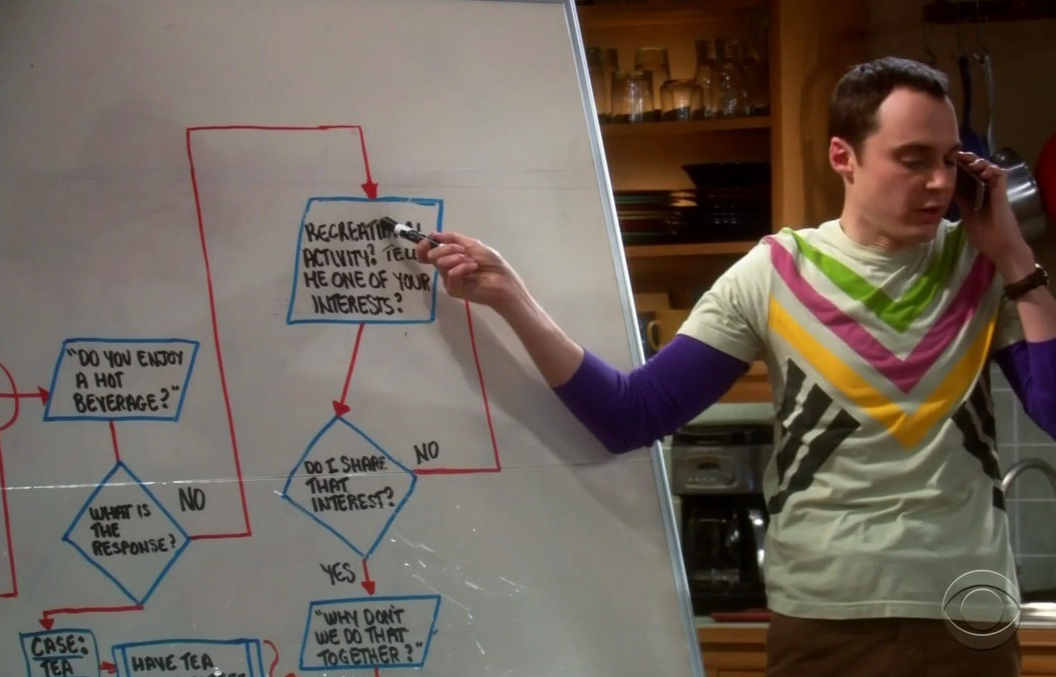
\includegraphics[width=7cm]{fig/Algorithm-sheldon.png}
      \textit{``I believe I've isolated the algorithm for making friends.''}
      \small{
        \hfill Sheldon Cooper, 
        \hfill in \textit{The Big Band Theory}, Season 2, Episode 13
      }
    }
  \end{columns}
  
\end{frame}

%%%%%%%%%%%%%%%%%%%%% 

\subsection{Introduction}
\begin{frame}
  \frametitle{Pourquoi faire appel � des algorithmes ?}
  Pour automatiser des t�ches
  
  Exemples :
  \begin{itemize}
  \item M�tier � tisser\\
  \item M�thode de calcul � la main d'une division\\
  \item Recette de cuisine\\
  \item ...\\
  \end{itemize}
\end{frame}

%%%%%%%%%%%%%%%%% 

\begin{frame}
  \frametitle{Qu'est-ce qu'un algorithme ?}
  \begin{alertblock}{D�finition}
    Un algorithme est un ensemble 
    ordonn� d'instructions simples
    permettant de r�soudre un probl�me.
  \end{alertblock}
\end{frame}

%%%%%%%%%%%%%%%%%% 

\begin{frame}
\frametitle{Remarques}
  \begin{block}{Un algorithme n�cessite :}
    \begin{itemize}
    \item Des objets sur lesquels travailler,\\
    \item Un langage non ambigu,\\
    \item Des sp�cifications (description de l'algorithme).\\
    \end{itemize}
  \end{block}
  
  \begin{block}{}
    Il n'existe g�n�ralement pas un unique algorithme pour traiter un probl�me.
  \end{block}
\end{frame}

%%%%%%%%%%%%%%%%%

\begin{frame}
  \frametitle{Historique}
  \begin{description}
\item[3�me si�cle avant JC] \textit{Livre VII des El�ments d'Euclide}
 \begin{columns}[T]
    \column{8cm}
D�termination du plus grand diviseur commun entre deux nombres :
PGCD(12,8)=4\\

 \column{4cm}
    \centering{
      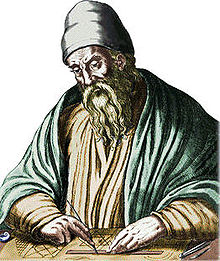
\includegraphics[width=4cm]{fig/Euclide.jpg}
}
\end{columns}
\item[8�me si�cle apr�s JC] \textbf{\textit{Al-Khawarizmi}} : M�thodes de r�solution d'�quations.
Son nom est � l'origine du mot "algorithme".
\end{description}
\end{frame}

%%%%%%%%%%%%%%%%%%%%%%%%%%%%%%%%%%%%%%%%%%%%%%%%%%%%%%%%%%%%%%%%%%%

\subsection{Construction d'un algorithme}

\begin{frame}
  \begin{columns}
    \column{4.8cm}
    \tableofcontents[currentsection,hideothersubsections,currentsubsection]
    \column{7cm}
    \centering{
      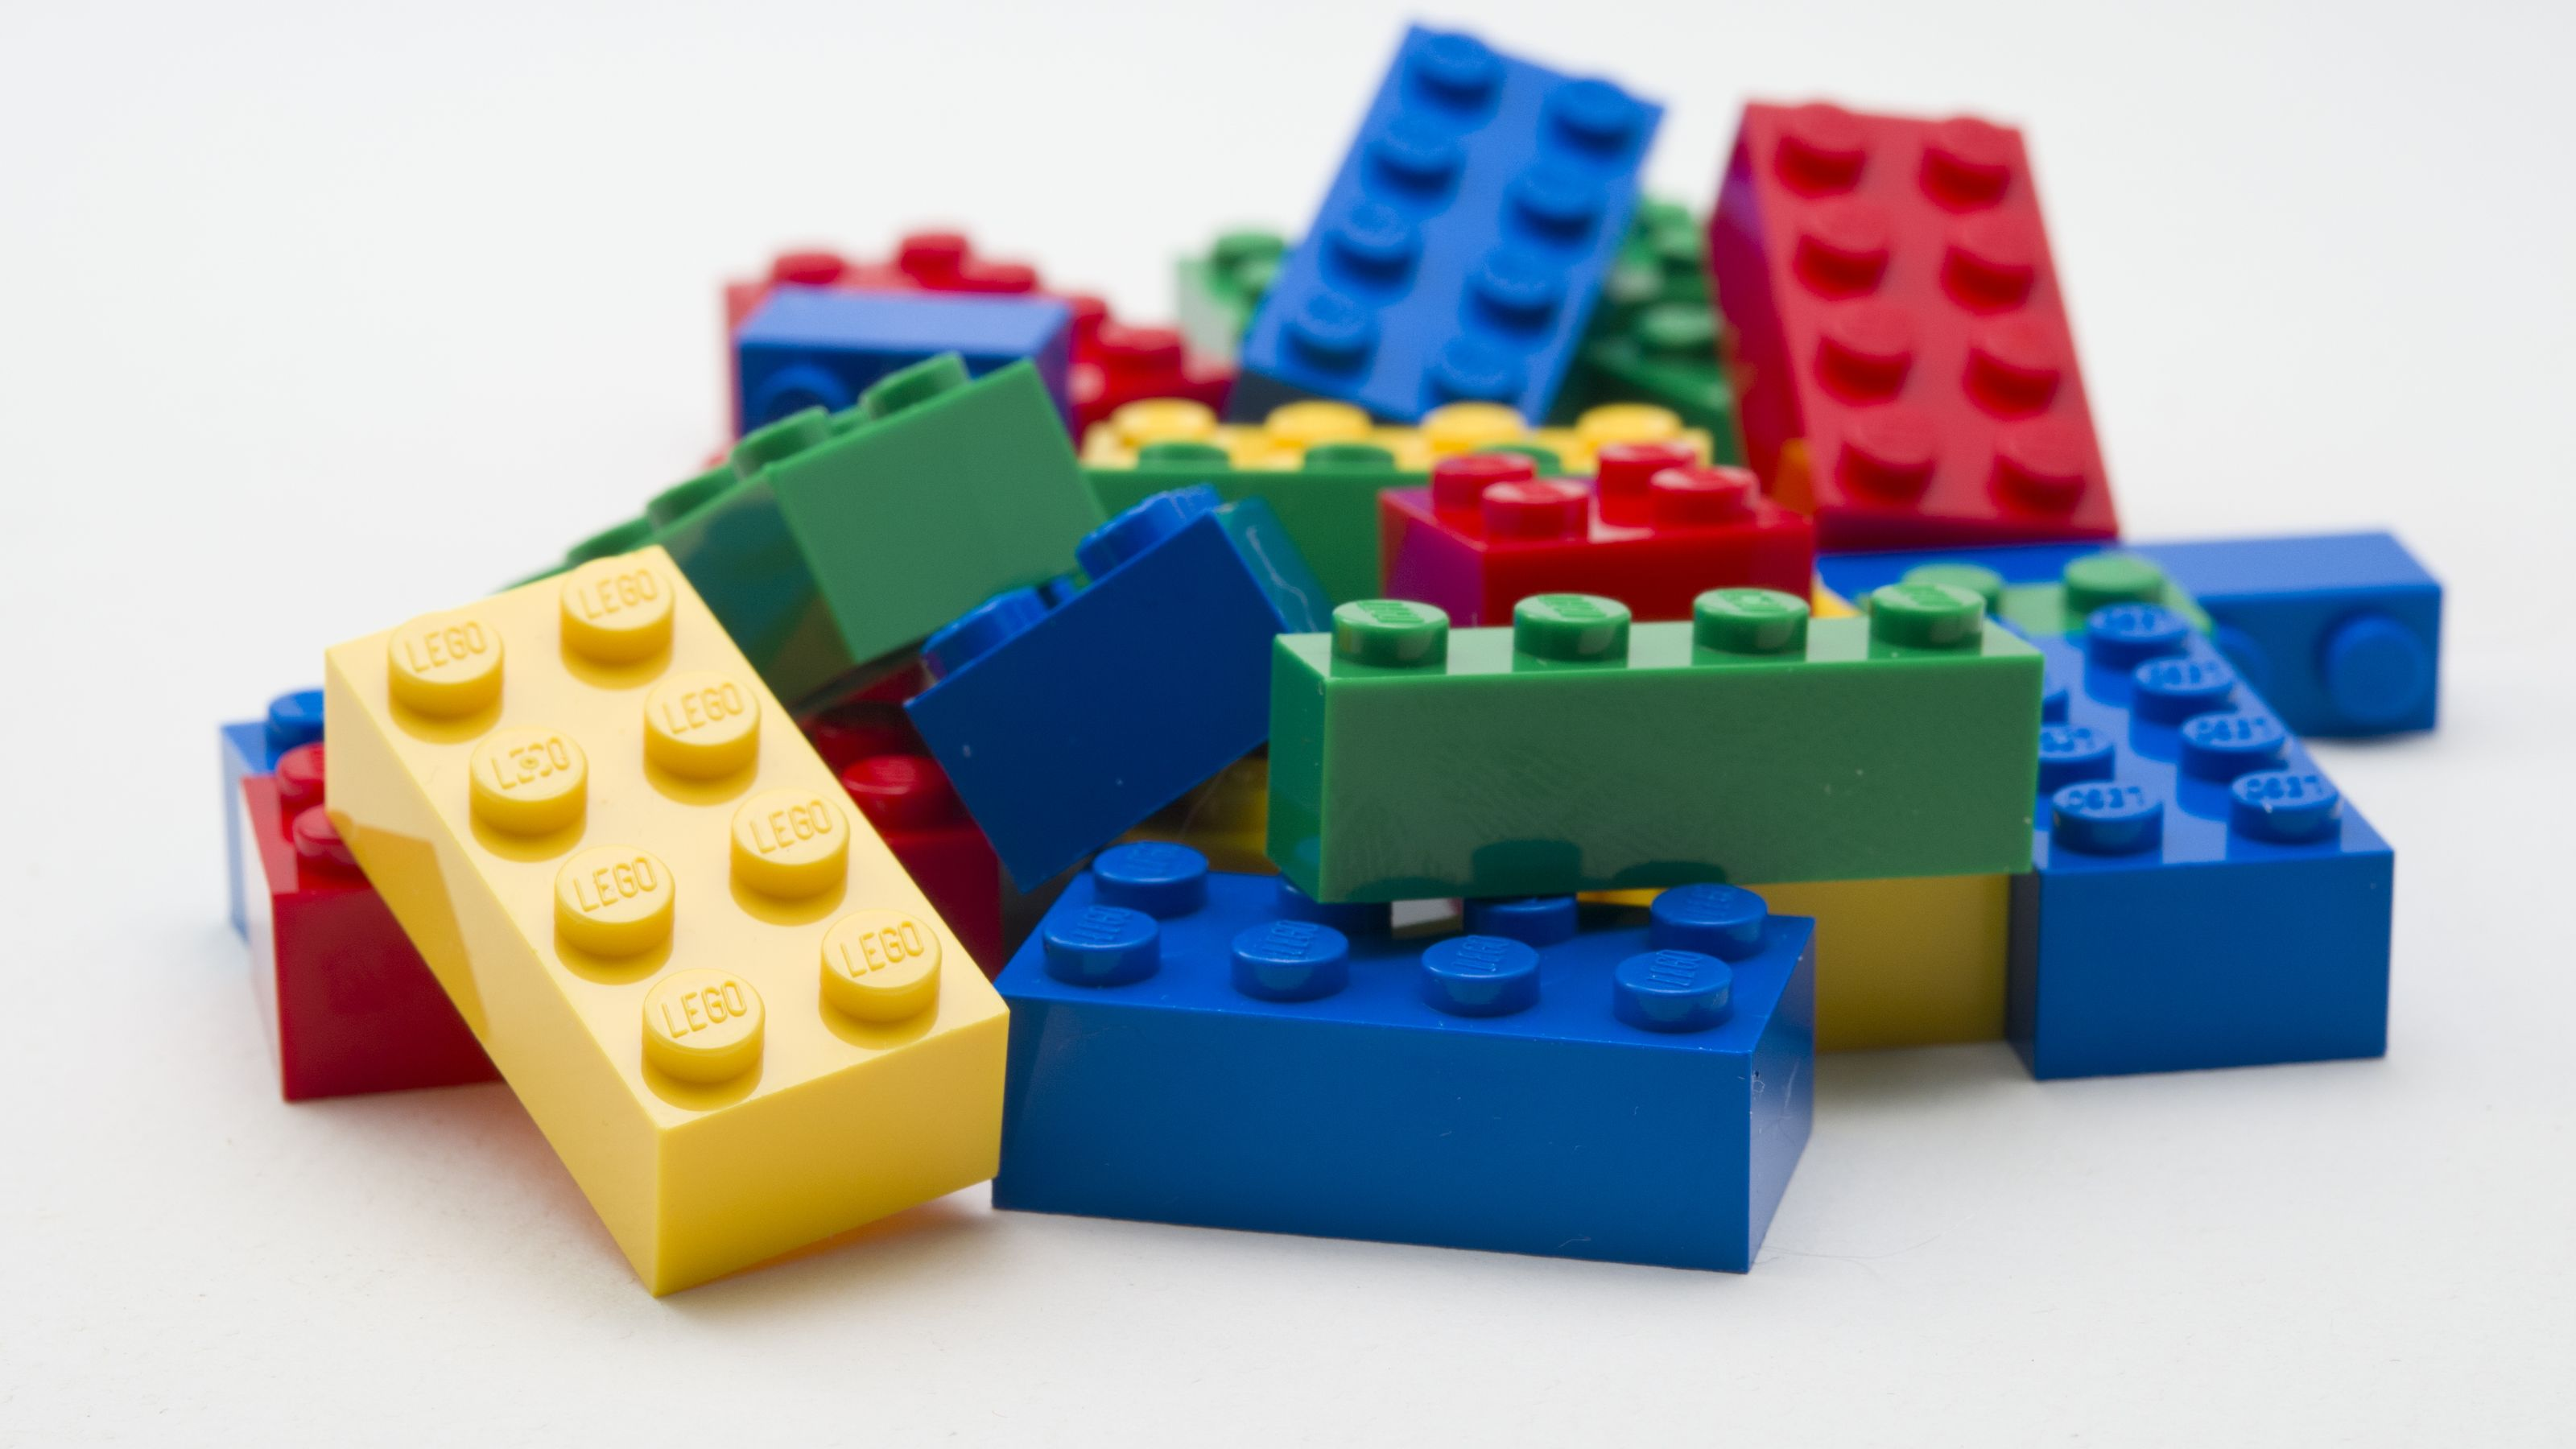
\includegraphics[width=7cm]{fig/lego.jpg}
     % \textit{``I believe I've isolated the algorithm for making friends.''}
     % \small{
     %   \hfill Sheldon Cooper, 
     %   \hfill in \textit{The Big Band Theory}, Season 2, Episode 13
%     }
    }
  \end{columns}
\end{frame}
 
%%%%%%%%%%%%%%%%%%%%%%%%%%%%%%%%%%%%%%%%%%%%%%%%%%%%%%%%%%%%%%%%%%%

\begin{frame}
  \frametitle{Construction d'un algorithme}
\begin{block}{Pour chaque probl�me, il vous est demand� de d�finir clairement :}
\begin{itemize}
\item Les �ventuelles \red{donn�es d'entr�e du probl�me} en pr�cisant leurs types et leur r�le,\\
\item les �ventuelles \red{donn�es de sortie du probl�me} en pr�cisant leurs types, \\
\item les diff�rentes \red{instructions} permettant d'obtenir les donn�es de sorties � partir
des donn�es d'entr�e.\\
\end{itemize}
\end{block}
\end{frame}

%%%%%%%%%%%%%%%%%%%%%%%%%%%%%%%%%%%%%%

\begin{frame}[fragile]
\frametitle{Exemple}
Algorithme qui d�termine le prix d'entr�e dans un mus�e (les mineurs payent moiti� prix)
\pause
\begin{columns}[t]
\column{6 cm}
\begin{exampleblock}{Donn�es}
\begin{algorithmic}[1]
\REQUIRE{age (entier)}\\
\COMMENT{age du client}
\ENSURE{tarif (d�cimal)}\\
\COMMENT{prix de l'entr�e}
\end{algorithmic}
\end{exampleblock}
\column{5 cm}
\pause

\begin{exampleblock}{Instructions}
\begin{algorithmic}[0]
\IF{age < 18}
\STATE tarif $\leftarrow$ 4
\ELSE
\STATE tarif $\leftarrow$ 8
\ENDIF
\RETURN{tarif}
\end{algorithmic}
\end{exampleblock}

\end{columns}
\end{frame}

%%%%%%%%%%%%%%%%%%%%%%%%%%%%%%%%%%%%%%%%%%%%%
\begin{frame}[fragile]
\frametitle{Structures conditionnelles 1/2}
\begin{columns}[t]
\column{6cm}
%\begin{block}

\begin{figure}
\begin{tikzpicture} [
    auto,
    decision/.style = { diamond, draw=blue, thick, fill=blue!20,
                        text width=1.5cm, text badly centered,
                        rounded corners, aspect=2 },
    block/.style    = { rectangle, draw=blue, thick, 
                        fill=blue!20, text width=1.5cm, text centered,
                        rounded corners, minimum height=2em },
    line/.style     = { draw, thick, ->, shorten >=2pt },
    node distance=1.5cm,
  ]
  \node (rac) {} ;
  \node (condition) [decision, below of=rac] {condition} ; 
  \node (center) [draw,circle,  thick, inner sep=2pt,minimum size= 0pt, radius = 2pt,below of =condition]{};
  \node (false) [block, left of=center,xshift=-3mm] {Action F};
  \node (true) [block, right of=center,xshift=3mm] {Action V};
   \node (end) [below of=center]{};
  % Define nodes in a matrix
  %\matrix [column sep=5mm, row sep=10mm] {
  %& \node (rac) {}; & \\
  %& \node [decision] (condition) {condition}; & \\
  %\node [block] (true) {Action V}; & & \node [block] (true) {Action V} ; \\
 % & \node (end) {}; \\
  %};
  
  % connect nodes
  \begin{scope}[every path/.style=line]
  \path (rac) -- (condition);
  \path (condition) -| node [near start, above] {vraie} (true);
  \path (condition) -| node [near start, above] {fausse} (false);
  \path (center) -- (end) ;
  %\path (false) -| (end);
  \end{scope}
  \draw[-, thick] (true) -- (center) ;
    \draw[-, thick] (false) -- (center) ;

\end{tikzpicture}
\end{figure}
%\end{block}
\column{5cm}

\begin{block}{}
\begin{algorithmic}[0]
\IF{\red{condition}}
\STATE Action V
\ELSE
\STATE Action F
\ENDIF
\end{algorithmic}
\end{block}

\begin{exampleblock}{Un exemple}
\begin{algorithmic}[0]
\IF{age < 18}
\STATE tarif $\leftarrow$ 4
\ELSE
\STATE tarif $\leftarrow$ 8
\ENDIF
\end{algorithmic}
\end{exampleblock}

\end{columns}
\end{frame}

\end{document}

%%%%%%%%%%%%%%%%%%%%% SECTION 1
\section{Les algorithmes}\label{section:1}
\begin{frame}
\begin{columns}
        \column{4.8cm}
            \tableofcontents[currentsection]
        \column{7cm}
        \centering{
            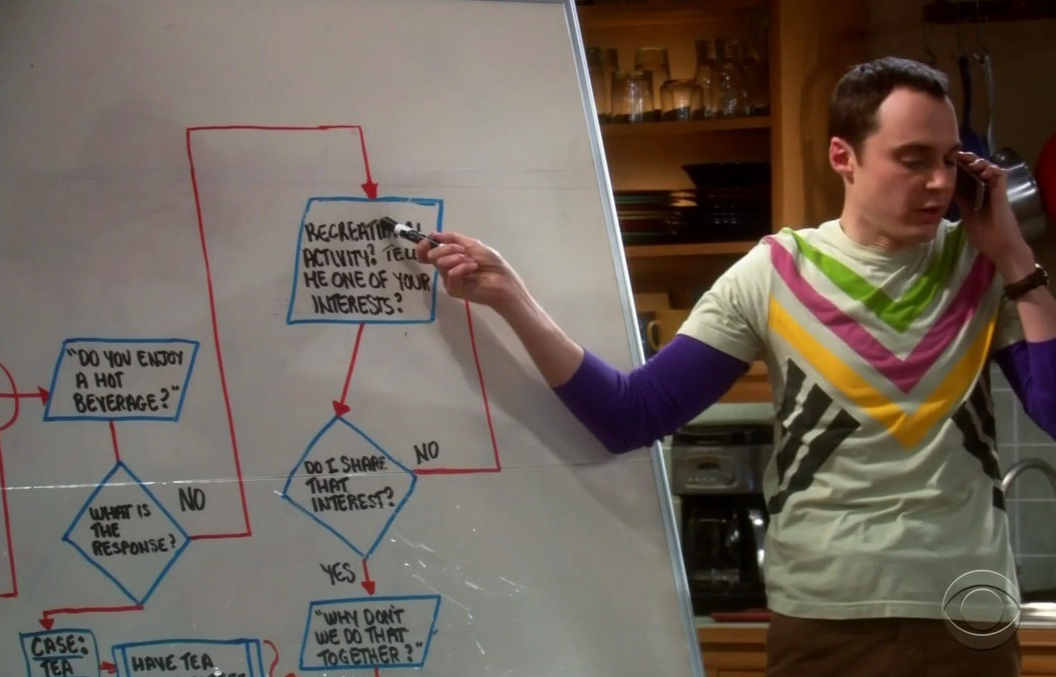
\includegraphics[width=7cm]{fig/Algorithm-sheldon.png}
            
                 \textit{ I believe I've isolateblblblblblblsblbslbslbsl
            sblbslblsblsblblsblbs
            lbslblbslsb d the algorithm for making friends.}
     
            
            \small{
            \hfill Sheldon Cooper, 
            
            \hfill in \textit{The Big Band Theory}, Season 2, Episode 13
            }
}

    \end{columns}

\end{frame}


%%%%%%%%%%%%%%%%%%%%%
\subsection{Introduction}
    \begin{frame}
    \frametitle{Pourquoi faire appel � des algorithmes ?}
    Pour automatiser des t�ches
    
    Exemples :
    \begin{itemize}
    \item M�tier � tisser\\
    \item M�thode de calcul � la main d'une division\\
    \item Recette de cuisine\\
    \item ...\\
    \end{itemize}
    \end{frame}
 
 %%%%%%%%%%%%%%%%%
 
    \begin{frame}
    \frametitle{Qu'est-ce qu'un algorithme ?}
    \begin{block}{D�finition}
    Un algorithme est un ensemble 
    ordonn� d'instructions simples
permettant de r�soudre un probl�me.
    \end{block}
    \end{frame}
    
 %%%%%%%%%%%%%%%%%%
 \subsection{Construction d'un algorithme}
%%%%%%%%%%%%%%%%%%%    
\section{La machine de Turing}
%%%%%%%%%%%%%%%%%%%%
 
  
\begin{frame}[fragile]
\frametitle{Un peu d'histoire...}
\begin{codeblock}{Test}
\begin{codeC}
for (int i = 0 ; i < n ; i ++) {
    //a comment
    printf("%d",i);
    }
\end{codeC}
\end{codeblock}

\begin{termblock}{test 2}
\lstset{escapeinside={��}}
\begin{lstlisting}
�\textbf{>>}�./a.out
�\color{darkgray}{\texttt{  Hello World}}�
\end{lstlisting}
\end{termblock}

 \begin{block}{Bloc standard}
blablabla
\end{block}
\end{frame}


\begin{frame}[fragile]
\frametitle{essai}
\begin{columns}
\column{6cm}
\begin{block}

\begin{figure}
\begin{tikzpicture} [
    auto,
    decision/.style = { diamond, draw=blue, thick, fill=blue!20,
                        text width=5em, text badly centered,
                        inner sep=1pt, rounded corners },
    block/.style    = { rectangle, draw=blue, thick, 
                        fill=blue!20, text width=10em, text centered,
                        rounded corners, minimum height=2em },
    line/.style     = { draw, thick, ->, shorten >=2pt },
  ]
   \matrix [column sep=-10mm, row sep=10mm] {
                    & \node [text centered] (x) {$\mathbf{X}$};            & \\
                    & \node (null1) {};                                    & \\
                    & \node [block] (doa) {\textsf{DoAE}($\mathbf{X}$)};   & \\
  	               \node(null3){}; & \node [decision] (uiddes)
                        {\textsf{UID}($\hat{\mathbf{X}}$)};
                                  & \node[text centered](tra){$\mathbf{i}$}; \\
                  & \node [block] (track) {\textsf{DoAT}($\mathbf{x}$)}; & \\
                    & \node [block] (pesos)
                        {\textsf{BF}(DoA$_{\mathrm{T}}$,DoAs)};            & \\
                    & \node [block] (filtrado)
                        {\textsf{SF}($\mathbf{w}$,$\mathbf{x}$)};          & \\
                    & \node [text centered] (xf) {$\hat{x}(t)$ };          & \\
  };
  % connect all nodes defined above
 \begin{scope} [every path/.style=line]
    \path (x)        --    (doa);
    \path (doa)      --    node [near start] {DoAs} (uiddes);
    \path (tra)      --    (uiddes);
    \path (uiddes)   --++  (-3,0) node [near start] {no} |- (null1);
    \path (uiddes)   --    node [near start] {DoA} (track);
    \path (track)    --    node [near start] {DoA$_{\mathrm{T}}$} (pesos);
    \path (pesos)    --    node [near start] {\textbf{w}} (filtrado);
    \path (filtrado) --    (xf);
  
  \end{scope}
\end{tikzpicture}
\end{figure}
\end{block}
\column{3cm}
\begin{block}{bulbul}
\end{block}
\end{columns}
\end{frame}


\end{document}
